%\documentclass[10pt,conference]{IEEEtran}
%\IEEEoverridecommandlockouts
% The preceding line is only needed to identify funding in the first footnote. If that is unneeded, please comment it out.

\documentclass[sigconf,review,anonymous]{acmart}

\AtBeginDocument{%
  \providecommand\BibTeX{{%
    \normalfont B\kern-0.5em{\scshape i\kern-0.25em b}\kern-0.8em\TeX}}}

\setcopyright{acmcopyright}
\copyrightyear{2023}
\acmYear{2023}
\acmDOI{XXXXXXX.XXXXXXX}

%% These commands are for a PROCEEDINGS abstract or paper.
\acmConference[ICSE 2024]{46th International Conference on Software Engineering}{April 2024}{Lisbon, Portugal}
%%
%%  Uncomment \acmBooktitle if the title of the proceedings is different
%%  from ``Proceedings of ...''!
%%
%%\acmBooktitle{Woodstock '18: ACM Symposium on Neural Gaze Detection,
%% June 03--05, 2018, Woodstock, NY}
\acmPrice{15.00}
\acmISBN{978-1-4503-XXXX-X/18/06}


%\IEEEoverridecommandlockouts
% The preceding line is only needed to identify funding in the first footnote. If that is unneeded, please comment it out.
% \usepackage{cite}
 \usepackage{amsmath,amsfonts}
% \usepackage{algorithmic}
% \usepackage{graphicx}
 \usepackage{textcomp}
% \usepackage{xcolor}
\usepackage{xspace}
%\usepackage{float}
%\usepackage{balance}
%\usepackage{rotating}
%\usepackage{multirow}
%\usepackage{needspace}
%\usepackage{microtype}
%\usepackage{bold-extra}
%\usepackage{geometry}
%\usepackage{varioref}
%\usepackage{listings}
\usepackage[normalem]{ulem} %emphasize still italic
%\usepackage{ucs}
%\usepackage{times}
\usepackage{url} %to allow line breaks in footnote url
\def\UrlBreaks{\do\/\do-}
%\usepackage{alltt}
%\usepackage{xfrac}
%\usepackage{subfigure}
%\usepackage{stmaryrd}   % for the \shortuparrow
%\usepackage{setspace}
%\usepackage[numbers, sort&compress]{natbib}
%\usepackage{mdwlist}        % support for better spaced lists
%\usepackage{chngpage} % allows for temporary adjustment of side margins
%\usepackage[normalem]{ulem}
\usepackage{subcaption}
\usepackage{tablefootnote}
\usepackage{array, booktabs}
\usepackage{blindtext}
%\PassOptionsToPackage{hyphens}{url}
%\usepackage[pdftex,colorlinks=true,pdfstartview=FitV,linkcolor=black,citecolor=black,urlcolor=black]{hyperref}
%\usepackage{hyperref}
\usepackage{ifthen}
%\usepackage[normalem]{ulem} % for \sout
%\usepackage{todonotes}
\usepackage[shortlabels]{enumitem}
%\usepackage{enumerate}

\usepackage{csvsimple}
\usepackage{supertabular} % for creating tables that can break across multiple pages. It works similarly to the longtable package but is designed to work well in multicolumn environments.
%\usepackage{multicol} %allow the table to break over columns
\usepackage[most]{tcolorbox}
%\usepackage[multiple]{footmisc}
%\usepackage[caption=false]{subfig}
%\usepackage{subfloat}

%\usepackage{arydshln} % for cdashline
%\usepackage{paralist} %to list extends of previous work
%deactivate indentation on new paragraphs
%\usepackage{parskip}
% for wrapping text in table cells
\usepackage{tabularx}
%\usepackage{longtable} %for longtables however it cause problems with two column mode
%--- for dividing references into sections
%\usepackage[
%natbib=true,
%]{biblatex}
%\addbibresource{scg.bib}

\usepackage{fontawesome}      % for icon next to scg URL next to author list on title page
\usepackage{adjustbox} 		% for vertical text in tables
\usepackage{pifont} 		% for crosses and ticks in tables


\newcolumntype{R}[2]{
    >{\adjustbox{angle=#1,lap=\width-(#2),margin*=0.4em 0em 0em 0em}\bgroup}
    l
    <{\egroup}
}
\newcommand*\rot{\multicolumn{1}{R{90}{1em}}} % no optional argument here, please!

% for footnotes 1,2,3..... style
% (traditional approach with \usepackage[multiple]{footmisc} breaks clickable links, overrides behavior)
\let\oldFootnote\footnote
\newcommand\nextToken\relax
\renewcommand\footnote[1]{%
    \oldFootnote{#1}\futurelet\nextToken\isFootnote}
\newcommand\isFootnote{%
    \ifx\footnote\nextToken\textsuperscript{,}\fi}

\renewcommand{\arraystretch}{1.2}

%-------------- background boxes for RQs-------------
\definecolor{gray50}{gray}{.5}
\definecolor{gray40}{gray}{.6}
\definecolor{gray30}{gray}{.7}
\definecolor{gray20}{gray}{.8}
\definecolor{gray10}{gray}{.9}
\definecolor{gray05}{gray}{.95}

\newlength\Linewidth
\def\findlength{\setlength\Linewidth\linewidth
	\addtolength\Linewidth{-4\fboxrule}
	\addtolength\Linewidth{-3\fboxsep}
}
\newenvironment{rqbox}{\par\begingroup
	\setlength{\fboxsep}{5pt}\findlength
	\setbox0=\vbox\bgroup\noindent
	\hsize=0.95\linewidth
	\begin{minipage}{0.95\linewidth}\normalsize}
	{\end{minipage}\egroup
	\textcolor{gray20}{\fboxsep1.5pt\fbox
		{\fboxsep5pt\colorbox{gray05}{\normalcolor\box0}}}
	\endgroup\par\noindent
	\normalcolor\ignorespacesafterend}
\let\Rqbox\rqbox
\let\endRqbox\endrqbox



\newcommand{\rb}[1]{
	
	%\vspace{0.3cm}
	\begin{tcolorbox}[colback=gray!05,%gray background
		colframe=black,% black frame colour
		width=\columnwidth,% Use 5cm total width,
		arc=3mm, auto outer arc,
		boxrule=0.5pt,
		]
		#1
	\end{tcolorbox}
}

\newcounter{Finding}
\stepcounter{Finding}

\newcommand{\roundedbox}[1]{
	\rb{
		\noindent
		\textit{\textbf{Finding \theFinding}. #1}
	}
	\stepcounter{Finding}
}

\newcommand{\needlines}[1]{\Needspace{#1\baselineskip}}
\newcommand{\ra}{$\rightarrow$}
\newcommand{\yellowbox}[1]{\fcolorbox{gray}{yellow}{\bfseries\sffamily\scriptsize#1}}
\newcommand{\triangles}[1]{{\sf\small$\blacktriangleright$\textit{#1}$\blacktriangleleft$}}
\newcommand{\nb}[2]{\nbc{#1}{#2}{orange}}
\newcommand{\here}{\yellowbox{$\Rightarrow$ CONTINUE HERE $\Leftarrow$}}
\newcommand\fix[1]{\nb{FIX}{#1}}

% add more author macros here
\newcommand\tk[1]{\nbc{TK}{#1}{olive}} 
\newcommand\ab[1]{\nbc{AB}{#1}{purple}}
\newcommand\pr[1]{\nbc{PR}{#1}{violet}}
\newcommand\jz[1]{\nbc{JZ}{#1}{brown}}
\newcommand\vk[1]{\nbe{VK}{#1}{red}}
\newcommand\rB[1]{\nbe{Reviewer 2}{#1}{blue}}
\newcommand\rC[1]{\nbe{Reviewer 3}{#1}{magenta}}
\newcommand\ANS[1]{\nbe{Response}{#1}{teal}}
\newcommand\todo[1]{\nb{TO DO}{#1}}


\newcommand\remind[1]{\nbc{REMINDER}{#1}{gray}}
\newcommand\review[1]{\nbc{TO REVIEW}{#1}{orange}}
\newcommand{\ie}{\emph{i.e.},\xspace}
\newcommand{\eg}{\emph{e.g.},\xspace}
\newcommand{\etal}{\emph{et al.}\xspace}
\newcommand{\etc}{\emph{etc.}\xspace}
\newcommand{\github}{{GitHub}\xspace}

\newcommand{\secheaderfield}[1]{\textbf{\code{#1}}}
%\newcommand{\SO}{{Stack Overflow}\xspace}

\newcommand{\darkui}{Dark UI Colors\xspace}
\newcommand{\dynretdel}{Dynamic Retry Delay\xspace}
\newcommand{\avoidextrawork}{Avoid Extraneous Work\xspace}
\newcommand{\raceidle}{Race-to-idle\xspace}
\newcommand{\openwneccesary}{Open Only When Necessary\xspace}
\newcommand{\pushpoll}{Push over Poll\xspace}
\newcommand{\powersave}{Power Save Mode\xspace}
\newcommand{\poweraware}{Power Awareness\xspace}
\newcommand{\reducesize}{Reduce Size\xspace}
\newcommand{\wificell}{WiFi over Cellular\xspace}
\newcommand{\suplog}{Suppress Logs\xspace}
\newcommand{\batchoper}{Batch Operations\xspace}
\newcommand{\cache}{Cache\xspace}
\newcommand{\decreaserate}{Decrease Rate\xspace}
\newcommand{\usrknowbest}{User Knows Best\xspace}
\newcommand{\informusr}{Inform Users\xspace}
\newcommand{\enoresolution}{Enough Resolution\xspace}
\newcommand{\sensorfusion}{Sensor Fusion\xspace}
\newcommand{\killtask}{Kill Abnormal Tasks\xspace}
\newcommand{\noscrinteraction}{No Screen Interaction\xspace}
\newcommand{\avoidgraphic}{Avoid Extraneous Graphics and Animations\xspace}
\newcommand{\mansyncod}{Manual Sync – On Demand\xspace}

\newcommand{\eps}{energy patterns\xspace}
\newcommand{\eaps}{energy antipatterns\xspace}
\newcommand{\EPS}{Energy Patterns\xspace}
\newcommand{\EAPS}{Energy Antipatterns\xspace}
\newcommand{\antipattern}{antipattern\xspace}
\newcommand{\antipatterns}{antipatterns\xspace}
\newcommand{\numberofpattensincode}{15\xspace}

\newcommand{\powergadget}{Intel Power Gadget\xspace}
\newcommand{\rapl}{Running Average Power Limit\xspace}
\newcommand{\drr}{DRD\xspace}
\newcommand{\oown}{OOWN\xspace}

\newcommand{\yes}{\ding{52}}
\newcommand{\no}{\ding{54}}

\newcommand{\smallfootnote}[1]{\footnote{\fontsize{6}{6}\selectfont #1}}
\newcommand{\n}{$\cdot$}
\newcommand{\y}{\checkmark}
\newcommand{\subscript}[1]{$_{\textrm{\footnotesize{#1}}}$}
\newcommand{\superscript}[1]{$^{\textrm{\footnotesize{#1}}}$}
\newcommand{\vertical}[1]{\raisebox{-4em}{\begin{sideways}{#1}\end{sideways}}}
\newcommand{\code}[1]{\texttt{#1}}
\newcommand{\paratitle}[1]{\emph{#1. }}

\newcolumntype{L}[1]{>{\raggedright\arraybackslash}m{#1}} % left aligned column

% given by IEEE template 
\def\BibTeX{{\rm B\kern-.05em{\sc i\kern-.025em b}\kern-.08em
    T\kern-.1667em\lower.7ex\hbox{E}\kern-.125emX}}
    
% ============================================================
% Markup macros for proof-reading
\newboolean{showedits}
\setboolean{showedits}{true} % toggle to show or hide edits
\ifthenelse{\boolean{showedits}}
{
	\newcommand{\meh}[1]{\textcolor{red}{\uwave{#1}}} % please rephrase
	\newcommand{\ins}[1]{\textcolor{blue}{\uline{#1}}} % please insert
	\newcommand{\del}[1]{\textcolor{red}{\sout{#1}}} % please delete
%	\newcommand{\chg}[2]{\textcolor{red}{\sout{#1}}{\ra}\textcolor{blue}{\uline{#2}}} % please change
	\newcommand{\chg}[2]{\textcolor{orange}{\uline{#2}}} % please change
	\newcommand{\nbe}[3]{
		{\colorbox{#3}{\bfseries\sffamily\scriptsize\textcolor{white}{#1}}}
		{\textcolor{#3}{\sf\small$\blacktriangleright$\textit{#2}$\blacktriangleleft$}}}
}{
	\newcommand{\meh}[1]{#1} % please rephrase
	\newcommand{\ins}[1]{#1} % please insert
	\newcommand{\del}[1]{} % please delete
	\newcommand{\chg}[2]{#2}
	\newcommand{\nbe}[3]{}
}

% ============================================================
% Box comments/edits
\ifthenelse{\boolean{showedits}}
{
	\newtcolorbox{inserted}{
		title=Inserted text:,
		colframe=blue,colback=blue!5!white,
		breakable,
		leftrule=0mm, 
		bottomrule=0mm,
		rightrule=0mm,
		toprule=0mm,
		arc=0mm, outer arc=0mm,
		oversize
	}
	\newtcolorbox{deleted}{
		title=Deleted text:,
		colframe=red,colback=red!5!white,
		breakable,
		leftrule=0mm, 
		bottomrule=0mm,
		rightrule=0mm,
		toprule=0mm,
		arc=0mm, outer arc=0mm,
		oversize
	}
	\newtcolorbox{refactored}{
		title=Rewritten text:,
		colframe=blue,colback=red!5!white,
		breakable,
		leftrule=0mm, 
		bottomrule=0mm,
		rightrule=0mm,
		toprule=0mm,
		arc=0mm, outer arc=0mm,
		oversize
	}
}{
	\newenvironment{inserted}{}{}
	\let\deleted\comment
	\newenvironment{refactored}{}{} 
}

% ============================================================
% Put edit comments in a really ugly standout display
\newboolean{showcomments}
\setboolean{showcomments}{true}
%\setboolean{showcomments}{false}
\ifthenelse{\boolean{showcomments}}
{\newcommand{\nbc}[3]{
		{\colorbox{#3}{\bfseries\sffamily\scriptsize\textcolor{white}{#1}}}
		{\textcolor{#3}{\sf\small$\blacktriangleright$\textit{#2}$\blacktriangleleft$}}}
	\newcommand{\version}{\emph{\scriptsize\id}}}
{\newcommand{\nbc}[3]{}
	\newcommand{\version}{}}

% ============================================================
% Constants
\newcounter{qcounter}

% ============================================================================
% Make quotes be italic
\renewenvironment{quote}
{\list{}{\rightmargin\leftmargin}
	\item\relax\begin{it}}
	{\end{it}\endlist}
\newcommand{\ttimes}{\ensuremath{\times}}

% =============================================================================
% Source Code
\definecolor{source}{gray}{0.9}
\lstset{
	language={},
	% characters
	tabsize=3,
	upquote=true,
	escapechar={^},
	keepspaces=true,
	breaklines=true,
	alsoletter={},
	breakautoindent=true,
	columns=fullflexible,
	showstringspaces=false,
	basicstyle=\footnotesize\ttfamily,
	% background
	frame=single,
	framerule=0pt,
	backgroundcolor=\color{source},
	% numbering
	%numbers=left,
	%numbersep=5pt,
	%numberstyle=\tiny,
	%numberfirstline=true,
	% captioning
	captionpos=b,
	numberbychapter=false,
	% formatting (html)
	moredelim=[is][\textbf]{<b>}{</b>},
	moredelim=[is][\textit]{<i>}{</i>},
	moredelim=[is][\uline]{<u>}{</u>}}
\newcommand{\ct}{\lstinline[backgroundcolor=\color{white},basicstyle=\footnotesize\ttfamily]}
\newcommand{\lct}[1]{{\small\tt #1}}

%----------------------------------------------------------------------------
% Custom macros
\newcommand\keyword[1]{[#1]}
% ============================================================
\newboolean{isblinded}
\setboolean{isblinded}{true}
%\setboolean{isblinded}{false}
\ifthenelse{\boolean{isblinded}}
{\newcommand\blind[1]{BLINDED\xspace}}
{\newcommand\blind[1]{#1\xspace}}


%\usepackage[pdftex,colorlinks=true,pdfstartview=FitV,linkcolor=black,citecolor=black,urlcolor=black,bookmarks=false]{hyperref}

%----------------------------------------------------------------------------
%Paper specific
\newcommand{\rqI}{To what extent can we adapt the energy patterns for mobile applications to web applications?}
\newcommand{\rqII}{What are the concerns and challenges of industry developers for energy patterns?}
\newcommand{\rqIII}{How does an energy pattern impact energy consumption?}

\newcommand{\repFolder}[1]{Folder ``\href{}{RP/#1}'' in the Replication package}
\newcommand{\repFile}[1]{File ``\href{}{RP/#1}'' in the Replication package}
%----------------------------------------------------------------------------




\begin{document}

\title{Appendix of ``Energy Patterns for Web: A Preliminary Study''}

\author{Authors details omitted for double-blind reviewing}

\begin{comment}
\author{Pooja Rani}
\email{rani@ifi.uzh.ch}
\orcid{0000-0001-5127-4042}
\affiliation{%
  \institution{University of Zurich}
  \city{Zurich}
  \country{Switzerland}
}

\author{Jonas Zellweger}
\affiliation{%
  \institution{University of Zurich}
  \city{Zurich}
  \country{Switzerland}
}

\author{Veronika Kousadianos}
\affiliation{%
 \institution{University of Bern}
 \city{Bern}
 \country{Switzerland}}

 \author{Luis Cruz}
 \email{L.Cruz@tudelft.nl}
\affiliation{%
 \institution{Software Engineering, TUDelft}
 \country{Netherlands}}
 
\author{Timo Kehrer}
\email{timo.kehrer@unibe.ch}
\affiliation{%
 \institution{University of Bern}
 \city{Bern}
 \country{Switzerland}}

\author{Alberto Bacchelli}
\email{bacchelli@ifi.uzh.ch}
\orcid{0000-0003-0193-6823}
\affiliation{%
  \institution{University of Zurich}
  \streetaddress{Binzm\"{u}hlestrasse 14}
  \city{Zurich}
  \state{ZH}
  \country{Switzerland}
  \postcode{8050}
}

\renewcommand{\shortauthors}{Rani et al.}
\end{comment}

\maketitle



% !TEX root = main.tex
\section{\texorpdfstring{$RQ_1$}: Adaptation of \EPS} 

For each pattern, we provide the original definition given by Cruz \etal, the adapted context for web applications, a solution, and an example \cite{cruz2019catalog}. The discussion part of each section can provide comparisons between mobile and web applications, examples, and research from other domains for that pattern. If the pattern only applies to a certain extent or in certain situations, the discussion aims to present the reasons and explanations.

\begin{table*}[tbh]
\footnotesize
	\begin{center}
		\caption{ Mobile \eps by Cruz \etal \cite{cruz2019catalog} with their description }
		\label{tab:patterns_description}
		\begin{tabular}{p{0.17\linewidth}p{0.77\linewidth}}
  \toprule
  			\textbf{Pattern} & \textbf{Description}\\\midrule
\darkui                           & Provide a dark UI color theme to save battery on devices with AMOLED screens.                                                                          \\
\dynretdel                      & Whenever an attempt to access a resource fails, increase the time interval before retrying to access the same resource.                                 \\
\avoidextrawork                   & Avoid performing tasks that are either not visible, do not have a direct impact on the user experience to the user or quickly become obsolete.         \\
\raceidle                            & Release resources or services as soon as possible (such as wake locks, screen).                                                                        \\
\openwneccesary                 & Open/start resources/services only when they are strictly necessary.                                                                                   \\
\pushpoll                          & Use push notifications to receive updates from resources, instead of actively querying resources (i.e., polling).                                      \\
\powersave                          & Provide an energy efficient mode in which user experience can drop for the sake of better energy usage.                                                \\
\poweraware                          & Have a different behavior when the device is connected/disconnected to a power station or has different battery levels.                                \\
\reducesize                              & When transmitting data, reduce its size as much as possible.                                                                                           \\
\wificell                      & Delay or disable heavy data connections until the device is connected to a WiFi network.                                                               \\
\suplog                           & Avoid using intensive logging.                                                                                                                         \\
\batchoper                         & Batch multiple operations instead of putting the device into an active state many times.                                                              \\
\cache                                   & Avoid performing unnecessary operations by using cache mechanisms.                                                                                     \\
\decreaserate                            & Increase time between syncs/sensor reads as much as possible.                                                                                          \\
\usrknowbest                         & Allow users to enable/disable certain features in order to save energy.                                                                                \\
\informusr                             & Let the user know if the app is doing any battery-intensive operations.                                                                                \\
\enoresolution                        & Collect or provide high-accuracy data only when strictly necessary.                                                                                    \\
\sensorfusion                            & Use data from low-power sensors to infer whether new data needs to be collected from high-power sensors.                                               \\
\killtask                     & Provide means of interrupting energy greedy operations (e.g., using timeouts or user input).                                                         \\
\noscrinteraction                    & Whenever possible, allow interaction without using the display.                                                                                         \\
\avoidgraphic & Graphics and animations are really important to improve the user experience. However, they can also be battery intensive ? use them with moderation.   \\
\mansyncod                 & Perform tasks exclusively when requested by the user.                                                                                                  \\ \hline
\end{tabular}
\end{center}
\end{table*}

% --------------------------------------------------------------------
\subsection{Dark UI Colors}\label{sec:patterns-DarkUIColors}
\textbf{Original:} {``}Provide a dark UI color theme to save battery on devices with AMOLED screens~\cite{cruz2019catalog}."

\paragraph{Adaptation to Web}\mbox{}

\textbf{Context:} Dark mode can be applied to anything with a GUI (graphical user interface - also sometimes referred to only as UI user interface). Since websites provide interactive GUIs, dark background colors can be applied to web UIs.

\textbf{Solution:} Provide a UI with dark background colors.

\textbf{Example:} There already exist websites that provide dark UI colors like wand.ai (see Figure \ref{fig:wandb} \footnote{\url{https://wandb.ai/site}}).
\begin{figure}
    \centering
    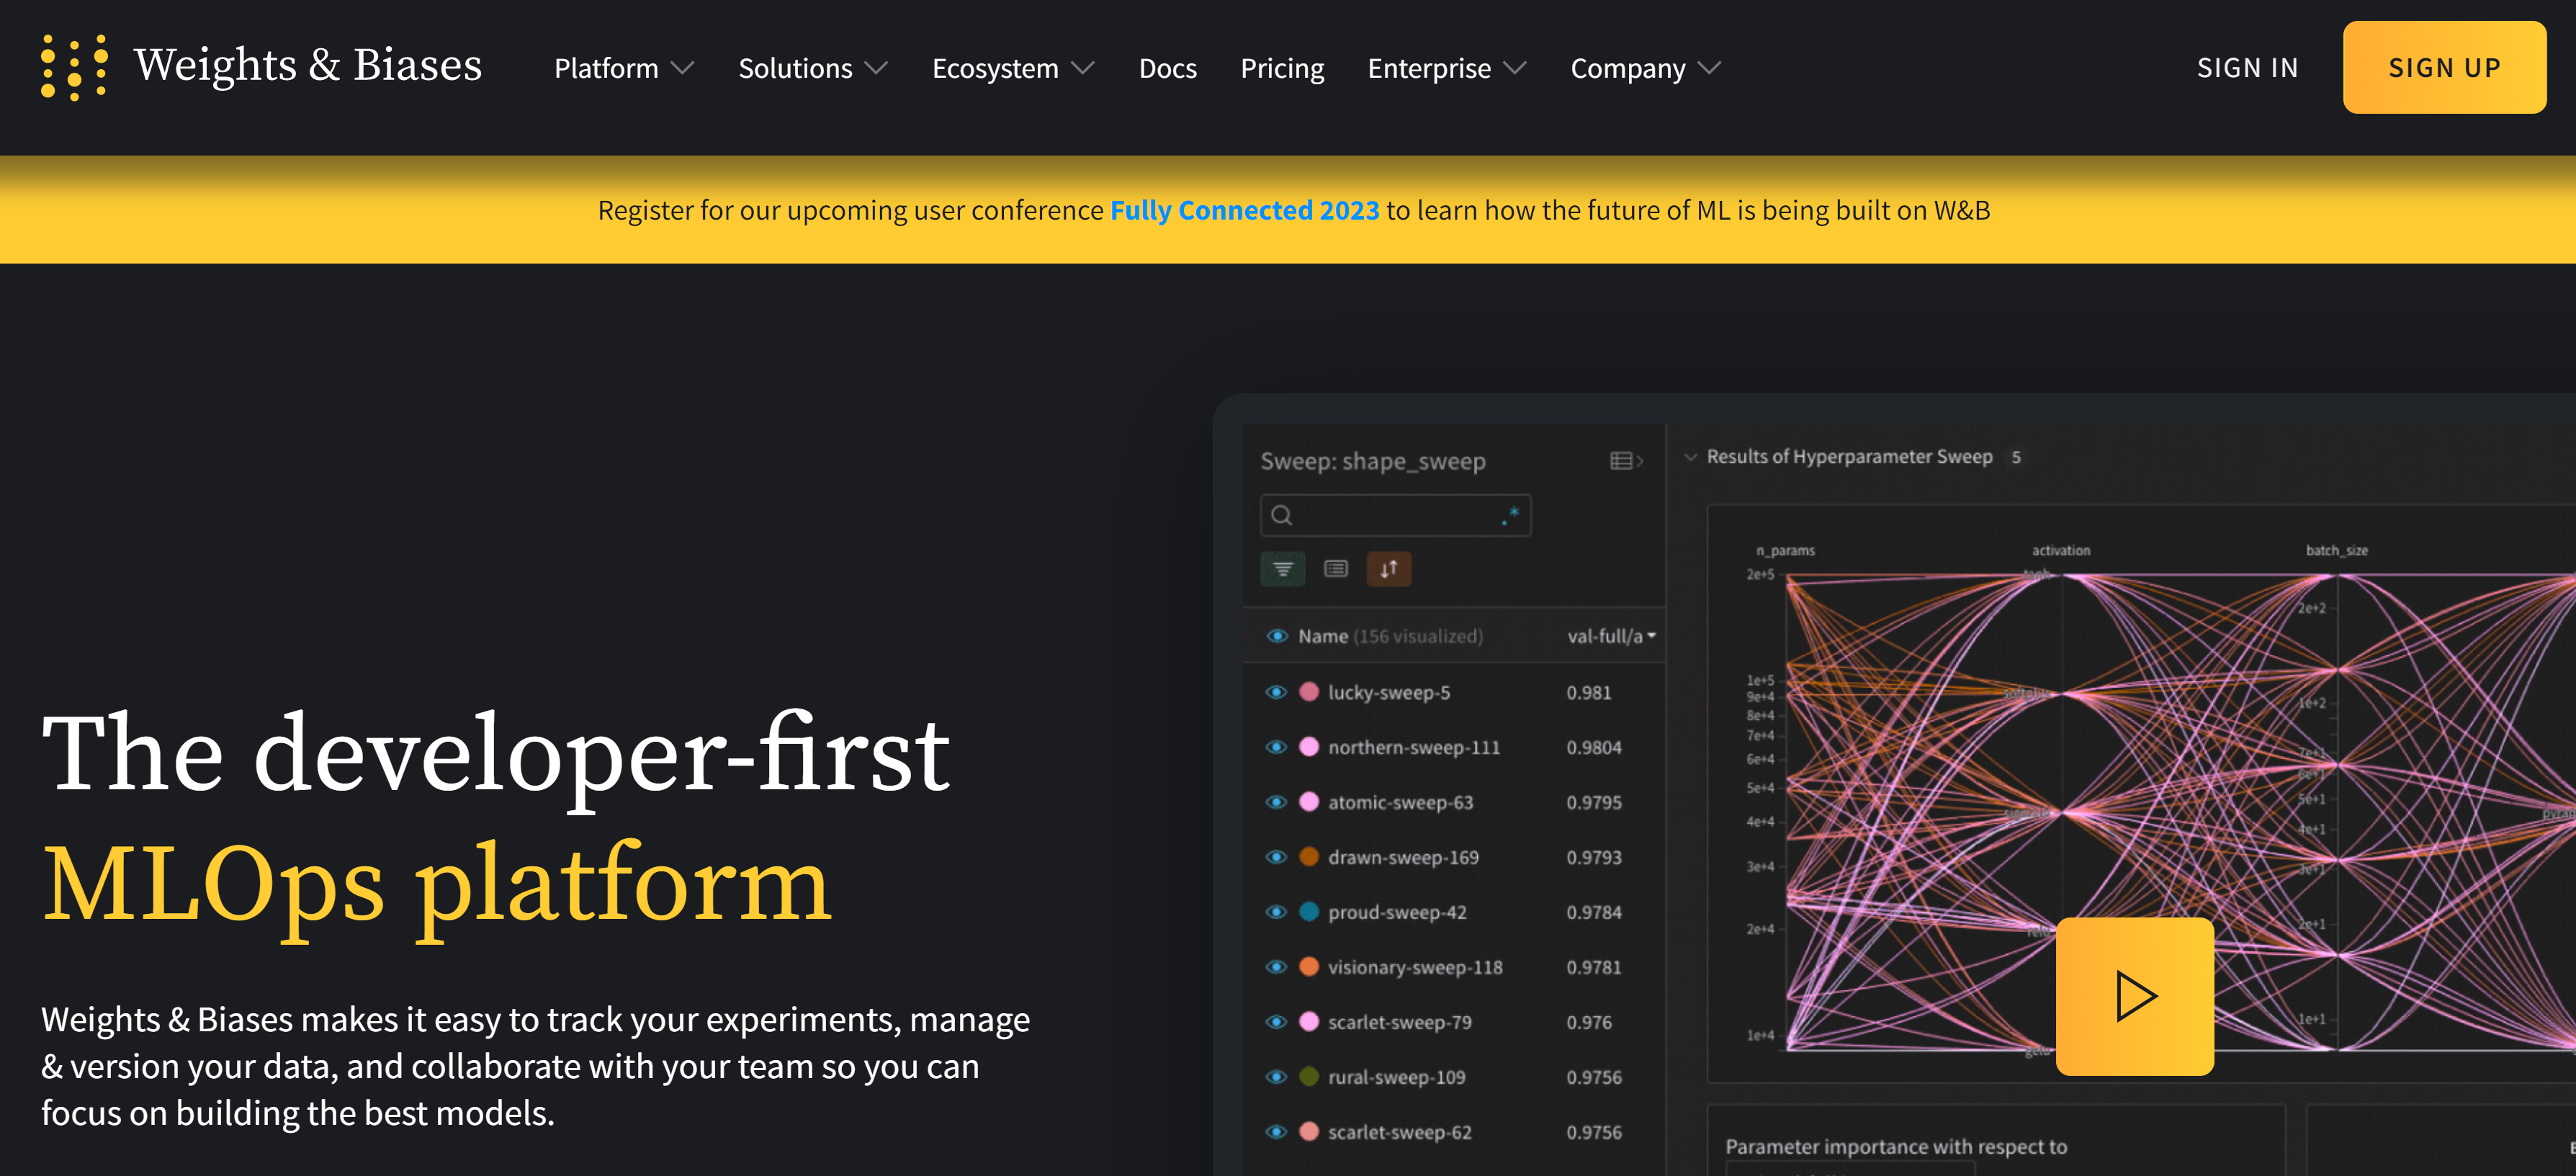
\includegraphics[width=\linewidth]{RQ1/Img/wandbAI.png}
    \caption{Screenshot of a website with dark UI colors.}
    \label{fig:wandb}
\end{figure}


\textbf{Discussion:} In mobile devices, the display alongside the GSM module are the two components with the highest power consumption ~\cite{Carroll2010}. Providing a dark UI color theme on devices with OLED (Organic Light Emitting Diodes) screens has been shown to reduce the display's power consumption up to 83\%, which can translate into a 69\% total phone power reduction~\cite{Dash2021}. This indicates that switching from light to dark mode saves a significant amount of battery.
The percentage of global web traffic recorded on mobile phones has increased drastically over the past decade. In February 2023, 60.67\% of all web traffic came through mobile phones \cite{statista}. Therefore, we expect similar benefits to battery life when accessing a web page with dark UI colors from a smartphone. To our knowledge, no research exists on energy consumption reduction of dark UI colors in non-battery-powered devices. We assume that depending on the monitor type used to display the web pages - namely, the newly emerging OLED monitors - there will be a reduction of energy consumption. Generally, we see dark UI colors catching on in web applications with motivations not only restricted to reducing power consumption: they range from adjusting brightness to current lighting conditions and improved display readability in dark environments~\cite{Mantiuk2009}~\cite{Rempel2012}, to having beneficial impact on users with reduced vision in certain circumstances~\cite{Bangor1999} and of course reduce power consumption on battery-powered devices~\cite{Dong2009}. Given this pattern's various benefits, it would be interesting to survey users to gather other possible benefits.

% --------------------------------------------------------------------
\subsection{Dynamic Retry Delay}\label{sec:patterns-DynamicRetryDelay}
\textbf{Original:} ``Whenever an attempt to access a resource fails, increase the time interval before retrying to access the same resource~\cite{cruz2019catalog}."

\paragraph{Adaptation to Web}\mbox{}

\textbf{Context:} The concept of managing retries to access a previously failed resource is a common topic across all computer science domains, including web applications. For instance, in client-server-based applications, the front and backend communication frequently happens through APIs. Specifically, the frontend sends a request to the backend, and based on the availability of the resource, the backend replies to the request.

\textbf{Solution:} Use a heuristic (\eg linear or exponential increase) to manage the retry interval after each failed attempt to connect.

\textbf{Example:} Consider a web application that displays a news feed. The frontend relies on the backend to provide updates. In case the frontend can not reach the backend, it can either continuously send requests to the backend or can increase the time between attempts using some sort of heuristic (\eg linear or exponential growth).  Listing \ref{dynamicretrydelaycode} shows an implementation utilizing the Fibonacci series to delay the retry attempts.

\begin{minipage}{0.95\linewidth}
    \begin{lstlisting}[caption={Example heuristics using the fibonacci series %\footnote{\url{https://github.com/hipjim/scala-retry}}
    },label={dynamicretrydelaycode}]
    val retryStrategy =
    RetryStrategy.fibonacciBackOff(initialWaitDuration = 3.seconds, maxAttempts = 5)
    \end{lstlisting}
\end{minipage}

\textbf{Discussion:} Research concerning the impact of energy consumption in connection with (re-)accessing resources is being conducted in different subdomains of computer science already. For example, in Wireless Sensor Networks (WSN), energy consumption is one of the main design constraints alongside scalability, delay, traffic adaptation, throughput, and overheads. Therefore, an efficient Medium Access Control (MAC) protocol is required~\cite{Kaur2016}. Cho \etal proposed a back-off algorithm for MAC protocols in WSN that uses a dynamic contention period based on the remaining energy (\ie battery level) of each sensor node~\cite{Cho2006}. They showed that this algorithm saves more power and prolongs the lifetime of sensor nodes compared to conventional back-off algorithms. We assume that using this and similar back-off algorithms would also decrease power consumption in other contexts, not only in wireless sensor networks.

A direct consequence of re-accessing a resource is that the end user experiences a delay while interacting with the application. Whenever a user experiences a delay in communication over a network, we speak of latency. Network latency can be described as the time it takes for a data package to travel from one point in the network to another.  There exists no agreement on what a good latency is. For example, an acceptable latency in gaming is around 40 - 60 milliseconds or less \cite{gaming_latency},
 while web domains accept values below 150 milliseconds for loading websites \cite{website_latency}
and below 100 milliseconds
when streaming videos or video conferencing \cite{latency-video}. This implies that as developers, we must be aware of the web application's purpose and aim for the maximum latency. While measuring the energy impact, we need to consider the sources, the domain, and the medium through which the internet is accessed as the latency is significantly lower when using an Ethernet connection compared to Wi-Fi \cite{ethernet-vs-wifi}. 

% --------------------------------------------------------------------
\subsection{Avoid Extraneous Work}\label{sec:patterns-AvoidExtraneousWork}
\textbf{Original:} ``Avoid performing tasks that are either not visible, do not have a direct impact on the user experience or quickly become obsolete~\cite{cruz2019catalog}."

\paragraph{Adaptation to Web}\mbox{}

\textbf{Context:} Web applications can perform a number of tasks simultaneously. There are cases in which the result of those tasks is either not visible (\eg the UI is presenting other pieces of information), or the result is not necessarily relevant to the user. This is particularly critical when the website goes to the background (\eg the user changes to another tab in the browser).

\textbf{Solution:} Investigate the relevant set of data to be presented to the user in each use case. Enable/disable updates and processing tasks depending on their effect on the visible or valuable data to the user.

\textbf{Example:} Consider the code snippet in \autoref{AvoidExtraenousWorkCode}. It shows an example where a website pauses audio when the user switches to a different tab and plays when they switch back. In this case, no unnecessary energy consumption will occur when the user is not interacting with the page.

\textbf{Discussion:} For web applications, for example, there exists the Page Visibility API \cite{MozillaAPI}. When the user switches to another tab or minimizes the window, this API sends an event to let listeners know that the state of the page has changed. This is especially useful for improving performance and also saving resources by not letting a page perform unnecessary tasks when the document isn't visible. See also the discussions in \ref{sec:patterns-OpenOnlyWhenNecessary} Open Only When Necessary and in \ref{sec:patterns-RaceToIdle} Race-to-idle.

In the context of web applications, its data, in the form of content, does not necessarily become as 'quickly obsolete' as in mobile applications. For example, recommendations based on location \eg for restaurants or for ATMs, will change if the user is on the move. Therefore, the location data from a couple of minutes ago can become obsolete. If we implement a mobile application, we expect the user to be on the move frequently. But if we implement a web application, we can not generally expect this behavior. Therefore, we recommend setting the focus of this pattern in web applications on tasks that are either not visible or do not directly impact the user experience.

\begin{minipage}{0.95\linewidth}
    \begin{lstlisting}[caption={Code snippet from Mozilla API that handles page visibility change},
     label={AvoidExtraenousWorkCode}]
    const audio = document.querySelector("audio");
    
    // Handle page visibility change:
    // - If the page is hidden, pause the video
    // - If the page is shown, play the video
    document.addEventListener("visibilitychange", () => {
      if (document.hidden) {
        audio.pause();
      } else {
        audio.play();
      }
    });
    \end{lstlisting}
\end{minipage}


% --------------------------------------------------------------------
\subsection{Race-to-idle}\label{sec:patterns-RaceToIdle}
\textbf{Original:} ``Release resources or services as soon as possible (such as wake locks, screen)~\cite{cruz2019catalog}."

\paragraph{Adaptation to Web}\mbox{}

\textbf{Context:} Releasing resources and services that are no longer needed is a very sensible coding practice that can be applied anywhere in computer science, including in web applications. The resources in the context of web applications refer to the backend, external servers, databases, and device hardware (\eg camera, microphone, and speaker).

\textbf{Solution:} Release unnecessary resources and services. This includes releasing the hardware resources that are no longer used (\eg camera after a video call) and applying resource management patterns (\eg garbage collection) during software development.

\textbf{Example:} Soundcloud uses React Redux in their techstack, which includes the functionality of garbage collection \cite{Garbagecollect}.

\textbf{Discussion:} There exist a number of resource management patterns in software development. For instance, Resource manager patterns \cite{design-pattern-resource-manager} for embedded and real-time systems utilize lists to keep track of free and busy resources to figure out how to allocate and free up resources in the system. Another common pattern is the dispose pattern \cite{wikipedia_dispose_pattern}, which is used across many object-oriented programming languages. Here, resources held by objects are released by calling methods like close(), release(), etc. This pattern is primarily used in those languages whose runtime environment have automatic garbage collection, such as C\# and Java. Other patterns regarding releasing resources include the \emph{Leasing pattern} and the \emph{Evictor pattern} \cite{resource-manager-patterns}.
For web application development, resource management patterns can be used in both front- and backend. According to intellipaat.com \cite{best-web-dev-languages}, the 4 most popular languages for backend development in web applications are Python, php, Java, and C\#, all of which support garbage collection. The most used language for the frontend is JavaScript along with its frameworks including Angular, React, and VueJS. JavaScript also supports garbage collection as a form of memory management \cite{dev_mozilla_memory_management}.

Browsers can promote similar behavior in websites themselves. WebKit \cite{webkit-website}, a web browser engine used by Safari and other apps on macOS, iOS, and Linux, automatically displays the following behavior when a page becomes inactive: 
\begin{itemize}
    \item window.requestAnimationFrame() is stopped,
    \item CSS and SVG Animations are halted,
    \item Timers are suspended \footnote{\url{https://webkit.org/blog/8970/how-web-content-can-affect-power-usage/}}.
\end{itemize}


% --------------------------------------------------------------------
\subsection{Open Only When Necessary} \label{sec:patterns-OpenOnlyWhenNecessary}
\textbf{Original:} ``Open/start resources/services only when they are strictly necessary~\cite{cruz2019catalog}."

\paragraph{Adaptation to Web}\mbox{}

\textbf{Context:} In web applications, some resources require to be opened before using them. In addition, there exist services and or resources that improve user experience but are non-critical. It is possible to open/load these resources and services at the very start when accessing the web page for the first time. However, the resources will actively wait for events or requests and passively consume energy even though they are not in use.

\textbf{Solution:} When accessing hardware, open resources only when necessary. During software development, identify non-critical services and load those only when necessary.

\textbf{Example:} A web application opens the camera only when necessary for capturing an image - not earlier when the application has been started (see \autoref{OpenOnlyWhenNecessaryCode}). Another example can be found in \autoref{OpenOnlyWhenNecessaryCode2}. It shows how images can be loaded lazily in web applications.

\begin{minipage}{\linewidth}
    \begin{lstlisting}[caption={Code snippet showing the usage of the loading attribute to lazy-load images \cite{lazy-loading-code-example}}, label={OpenOnlyWhenNecessaryCode2}]
img src=``image.png'' loading=``lazy'' alt=``...'' width=``200'' height=``200''
\end{lstlisting}
\end{minipage}

\textbf{Discussion:} Various hardware resources are available to websites, \eg a camera, microphone, and speaker. There exist APIs, \eg the Media Capture and Streams API (Media Stream) \cite{media-streams-api}, which allow developers to manipulate audio- or video-related data, including the access of said hardware.

In frontend development, there exists a widely used pattern called lazy loading. It allows for identifying non-critical resources and loading them only when necessary, avoiding unnecessary energy consumption. In addition, Tuaycharoen \etal show that lazy loading can increase the performance of web applications by 50\% due to an improved response time~\cite{Tuaycharoen2018}. The web application can use lazy loading in different scenarios and places. One typical use case happens during user interactions, such as scrolling and navigating.

\begin{minipage}
    \begin{lstlisting}[caption={Accessing the camera only when actually capturing the image - not earlier 
    %\footnote{\url{https://github.com/jbull328/vue-cam-demo/blob/master/src/components/CameraDisplay.vue} last accessed February 23}
    }, label={OpenOnlyWhenNecessaryCode}]
<template>
    ...
    <div  class="camera-icon" @click="captureImage">
        <i class="big camera icon" ></i>
        <p>Take Picture</p>
    </div>
    ...
</template>

<script>
    ...
    methods: {
        captureImage() {
            const mediaStreamTrack = this.mediaStream.getVideoTracks()[0]
            const imageCapture = new window.ImageCapture(mediaStreamTrack)
            let reader = new FileReader();
            return imageCapture.takePhoto().then(blob => {
                reader.readAsDataURL(blob)
                reader.onload = () => {
                    this.imageData.image = reader.result;
                }
            })  
        }
    }
    ...
    <\script>
    \end{lstlisting}
\end{minipage}

% --------------------------------------------------------------------
\subsection{Push over Poll} \label{sec:patterns-PushOverPoll}
\textbf{Original:} ``Use push notifications to receive updates from resources, instead of actively querying resources (\ie polling)~\cite{cruz2019catalog}."

\paragraph{Adaptation to Web}\mbox{}

\textbf{Context:} Handling updates from resources (\eg servers) is a crucial part of the web application design. Different approaches exist to get updates: the client repeatedly queries the server in set intervals to see if new data is available (\ie polling), or the server pushes new data to the client as soon as it is available. Since it is impossible to know if the server has new data available at this moment, the client continuously polling data will inevitably lead to unnecessary querying and thus may consume more energy.

\textbf{Solution:} Use the pushing mechanism to get updates from resources.

\textbf{Example:} Incorporate push notifications into the web application where possible. Listing \ref{pushoverpollcode} shows a possible implementation of such a push notification.

\begin{minipage}
    \begin{lstlisting}[caption={Code snippet of a push notification implementation.}, label={pushoverpollcode}]
public async Task SendNotificationAsync(PushSubscription subscription, 
    PushMessage message, CancellationToken cancellationToken)
{
    try
    {
        await _pushClient.RequestPushMessageDeliveryAsync(subscription, message, 
        cancellationToken);
    }
    catch (Exception ex)
    {
        await HandlePushMessageDeliveryExceptionAsync(ex, subscription);
    }
}
    \end{lstlisting}
\end{minipage}

\textbf{Discussion:} To avoid sending requests that will return no update in order to reduce unnecessary energy consumption is relevant for mobile applications since users rely on batteries. Ayala \etal found that using the polling mechanism consumes up to 10\% more energy than using long polling and up to 7.5\%  more energy for WebSocket in Android phones~\cite{Ayala2019}. When users access a web page from a mobile device, we would expect similar findings. To our knowledge, there exists no research about energy reduction comparing pulling and polling for non-mobile devices.

Web push notifications were introduced around 2015 by Google and Mozilla for Chrome 48 and Firefox 44, respectively. \footnote{\url{https://www.digitalmarketer.com/blog/use-web-push-notifications/}} They are widely used in e-commerce and social media to keep users engaged \cite{blog-web-push-notifications}. Downsides of push notifications for mobile applications have been researched by Kollmann \etal \cite{Kollmann2017}. The main concern is privacy since crucial information like the user's location (\ie IP address) is shared with the notification service. Similar issues could possibly affect web push notifications.

% --------------------------------------------------------------------
\subsection{Power Save Mode} \label{sec:patterns-PowerSaveMode}
\textbf{Original:} ``Provide an energy efficient mode in which user experience can drop for the sake of better energy usage~\cite{cruz2019catalog}."

\paragraph{Adaptation to Web}\mbox{}

\textbf{Context:} Providing energy efficient modes in which some functionalities are restricted or even dropped entirely can be implemented for any application (mobile and web).

\textbf{Solution:} Offer an energy-efficient mode in which the application consumes less energy.

\textbf{Example:} BooHoo has introduced an energy-saving mode to its website (see Figure \ref{fig:boohoo}).

\begin{figure}
    \centering
    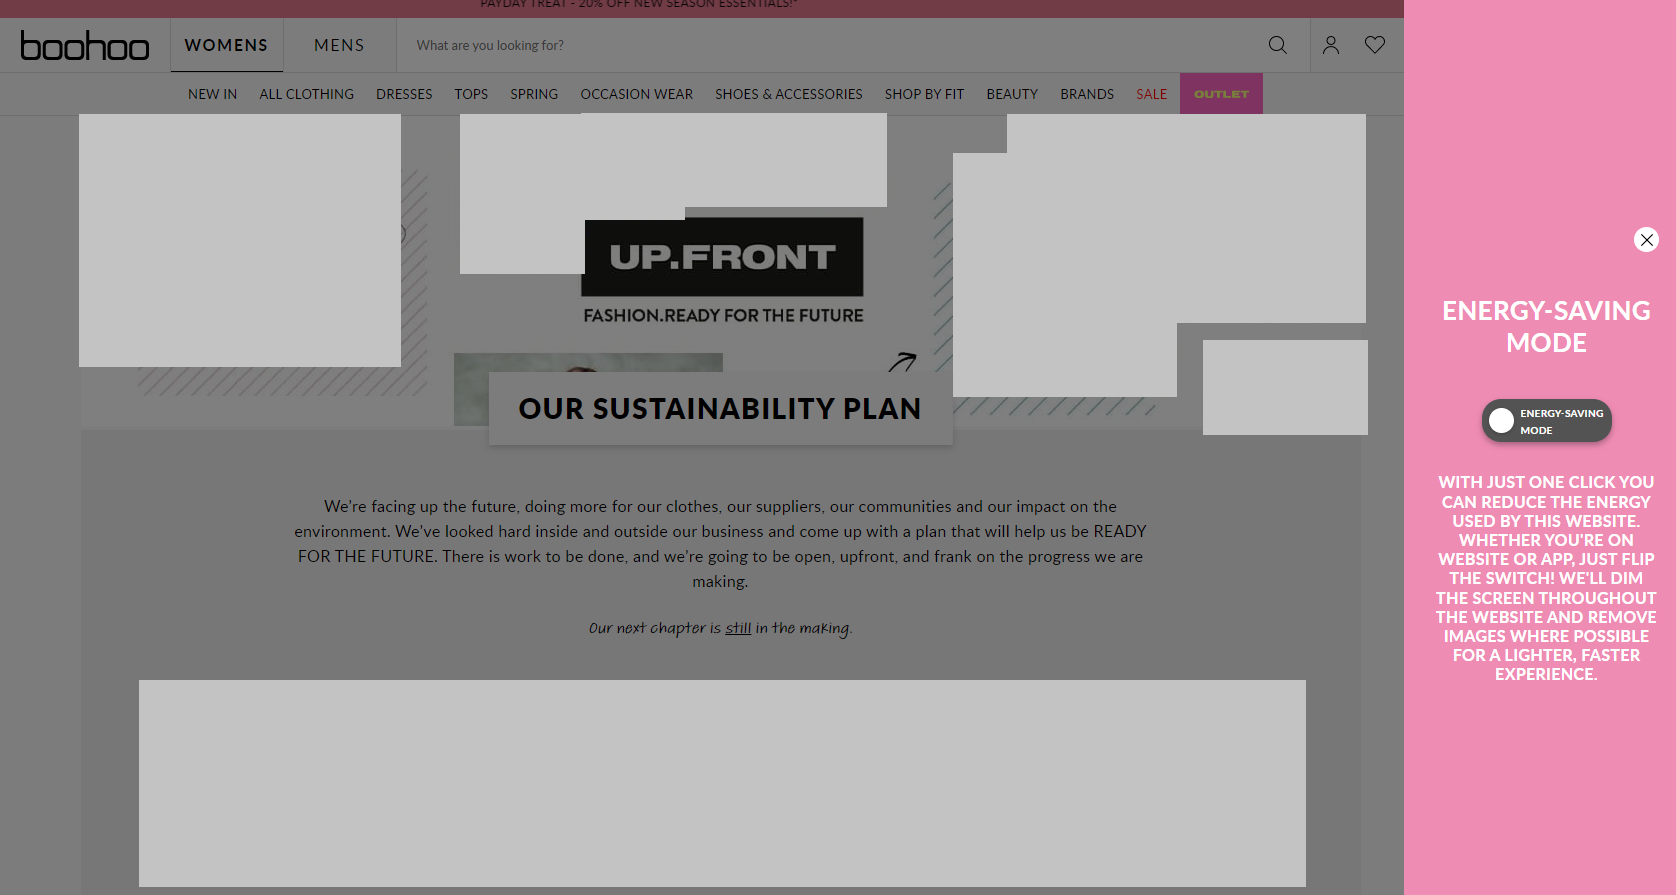
\includegraphics[width=\linewidth]{RQ1/Img/boohoo.png}
    \caption{Screenshot of a website with energy-saving mode \cite{boohoo-website}.}
    \label{fig:boohoo}
\end{figure}

\textbf{Discussion:} Providing energy-efficient modes in which some functionalities are restricted or even dropped entirely can be implemented for any mobile or web-based application. Using such an energy-efficient mode should reduce energy usage in any scenario. However, unless the user is on a device powered by a battery, they are unlikely to notice a reduction in energy consumption. 

Web applications are accessed via browsers. While browsers are not web applications themselves, they can play a crucial role in controlling the energy consumption of websites by potentially allowing web applications to provide energy-saving modes. As of February 2023, Google Chrome has been reported to perform testing on functionality that allows websites to switch to battery-saving mode \cite{chrome_battery_saving_mode} \cite{github_battery_saving_demo}. The browser Opera offers a battery-saving mode that reduces energy consumption when browsing any website, even in non-battery powered devices \cite{opera-battery-saver}. We conclude that there is a growing awareness of power-saving modes in the web application domain.

% --------------------------------------------------------------------
\subsection{Power Awareness} \label{sec:patterns-PowerAwareness}
\textbf{Original:} ``Have a different behavior when the device is connected/disconnected to a power station or has different battery levels~\cite{cruz2019catalog}."

\paragraph{Adaptation to Web}\mbox{}

\textbf{Context:} If web applications are used by devices without battery this pattern is not applicable. However, assuming the device used to access the web application has a battery, there are ways of adapting the behavior of an application according to the battery level or if the device is connected/disconnected.

\textbf{Solution:} Enable or disable certain functionalities of the device according to its power status.

\textbf{Example:} VueUse, a collection of Vue composition utilities, provides a reactive Battery Status API \cite{vueuse-useBattery}, which gives information about the system's battery level and charging status. For devices without battery, the boolean 'charging' will always be true.

\textbf{Discussion:} Websites can access information about the system's battery charge level through various APIs, for example, framework-specific APIs like VueUse' \code{useBattery()} or more general ones like the Battery Status API \cite{dev-mozilla-battery-status-api}, which uses the built-in \texttt{window.navigator} property of the navigator object in web pages. Thus, it is possible for developers to implement different behavior depending on the battery level of the device. Concerns have been raised that companies may utilize this information to their benefit and monetize access to battery levels. When the battery is running low, users might make different decisions than otherwise.\footnote{Podcast Episode 'Your Brain on Uber' on the Hidden Brain Podcast released in May 2016, accessed in March 2023}

Chrome has introduced a new feature called Energy Saver \cite{chrome-new-feature}, which limits background activity and visual effects (\eg animations and videos) as soon as the battery of the device reaches 20\%. Similarly, the aforementioned battery saving mode for the Opera browser can be configured to turn on automatically when the device is removed from the power station and, when unused, will send a reminder once the battery reaches 20\% that the mode is available \cite{opera-battery-saver}.

% --------------------------------------------------------------------
\subsection{Reduce Size} \label{sec:patterns-ReduceSize}
\textbf{Original:} ``When transmitting data, reduce its size as much as possible~\cite{cruz2019catalog}."

\paragraph{Adaptation to Web}\mbox{}

\textbf{Context:} Data transmission over a network is a routine operation in web applications, which can be energy greedy.

\textbf{Solution:} Transmit only what is necessary; avoid sending unnecessary data. Use data compression.

\textbf{Example:} Consider using headers \emph{Accept-Encoding} and \emph{Content-Encoding} for HTTP requests. Listing \ref{reducesizecode} shows an implementation where strings bigger than 1KB get compressed.


\textbf{Discussion:} Data transmission is a routine operation in web applications. Moreover, such operations can be energy greedy. The International Energy Agency (IEA) estimated the global internet traffic of 2021 to be 3.4 ZB (1 zetabyte = 10\textsuperscript{21} bytes), which has led to an increase of up to 60\% in the global data transmission network energy use since 2015 \cite{data_transmission_of_data_centers}. Reducing internet traffic can be achieved by compressing data before transmission. However, the work of Barr \etal ~\cite{Barr2006}  shows that in some cases, there can be a net energy increase when compression is applied before transmission. The energy consumption difference depends on hardware factors such as the relative energy of CPU, memory, and network, as well as software factors, including compression ratio and memory access patterns. In their work, the authors have measured up to 31\% overall energy reduction when using adequate compressors and decompressors for sending compressed web data~\cite{Barr2006}.

Not only can the data itself be compressed, but the request as a whole can be further optimized. Tools commonly used to make HTTP requests in web applications include XMLHttpRequest (XHR), Jquery Ajax, Fetch, Axios and Angular HttpClient \cite{Angular_Http_Client}. Using these packages allows developers to edit and adapt the requests being sent in their application, which allows, for example, the removal of unnecessary headers.

\begin{minipage}{0.95\linewidth}
    \begin{lstlisting}[caption={Impelemtation of data compression on strings larger than 1KB.
    %\footnote{\url{https://medium.com/axiomzenteam/put-your-http-requests-on-a-diet-3e1e52333014} last accessed April 23}
    }, label={reducesizecode}]
import axios from 'axios';
import pako from 'pako';

const api = axios.create({
  baseURL: "http://localhost:9000/api",
  withCredentials: true,
  transformRequest: axios.defaults.transformRequest.concat(
    function (data, headers) {
      // compress strings if over 1KB
      if (typeof data === 'string' && data.length > 1024) {
        headers['Content-Encoding'] = 'gzip';
        return pako.gzip(data);
      } else {
        headers['Content-Encoding'] = undefined;
        return data;
      }
    }
  )
});
    \end{lstlisting}
\end{minipage}

% --------------------------------------------------------------------
\subsection{Suppress Logs} \label{sec:patterns-SuppressLogs}
\textbf{Original:} ``Avoid using intensive logging ~\cite{cruz2019catalog}."

\paragraph{Adaptation to Web}\mbox{}

\textbf{Context:} Logging is common practice in web applications. Therefore, suppressing logs can be applied.

\textbf{Solution:} Refrain from extensive logging. Keep the logging rates below one message per second.

\textbf{Example:} The console output in Listing \ref{suppresslogscode} shows an example of possible logs. The logging level is \textit{warning}. This logging level includes warnings, errors, and critical system failures.

\begin{minipage}
    \begin{lstlisting}[caption={Console log of an interaction with a web application on log level warning. Other logging levels include warnings, errors, and critical system failures.}, label={suppresslogscode}]
# loglevel = warning

backend  | 2023-07-19 13:48:56,133 model_factory Response to request with pk 1234-5678-abcd 
    has content type text/javascript but was unable to parse it

backend  | 2023-07-19 13:49:02,343 model_factory Response to request with pk abcd-1234-5678 
    has content type text/javascript but was unable to parse it

backend  | 2023-07-19 13:49:12,876 model_factory Response to request with pk 1234-abcd-5678 
    has content type text/javascript but was unable to parse it
    \end{lstlisting}
\end{minipage}

\textbf{Discussion:} Shaiful \etal found, that execution logs for debugging can influence energy consumption in Android applications~\cite{Shaiful2018}. They show that the generation of logs at rates of one message per second or more negatively impacts energy consumption. Logging is one of the basic functionalities of most web applications. It records valuable information for operating and maintaining the website, such as the running information, user operations, debugging, warnings, and error information of the application~\cite{Pan2022}. To our knowledge, no study exists on the energy impact of logging in web applications. However, we assume, that extensive logging can also impact power consumption in web applications. Further, web applications are usually deployed in production mode, which by design does not support debugging. Therefore, the number of debugging logs in deployed websites will be zero. Thus eliminating the possibility of higher energy consumption caused by debugging logs. However, there are still logs available in production mode. There exist different logging levels: critical, error, warning, info, and debug are among the most common ones \cite{python-docs-logging}. The impact of continuously logging for different purposes on the server side or in source code is yet to be investigated.

% --------------------------------------------------------------------
\subsection{Batch Operations} \label{sec:patterns-BatchOperations}
\textbf{Original:} ``Batch multiple operations, instead of putting the device into an active state many times~\cite{cruz2019catalog}."

\paragraph{Adaptation to Web}\mbox{}

\textbf{Context:} Batch processing is widely used in applications that contain tasks that can be executed without user interaction, also in web applications.

\textbf{Solution:} Combine multiple operations into a batch for processing. By bundling multiple tasks, the overall efficiency can be improved, and possible tail energy consumption (energy consumption related to starting and stopping resources) can be reduced.

\textbf{Example:} Use Job Scheduling APIs for managing multiple tasks.

\begin{minipage}
    \begin{lstlisting}[caption={Usage of job scheduling in implementation to be able to batch operations}, label={BatchOperationsCode}]
def start_process():
    _create_and_return_bills()

    some_job = django_rq.enqueue(_setup, jobs,
                                job_timeout=7200)
    bill_jobs = []

    # Generate bills using workers.
    for bill in list_of_bills:
        bill_jobs.append(
            django_rq.enqueue(_generate_bill, bill, 
                                some_job.id,
                                depends_on=some_job))
                              
    # Bills for user are calculated concurrently
    bill_jobs.append(django_rq.enqueue(
        set_total_costs_for_billing, 
        all_bills, depends_on=bill_jobs))
    django_rq.enqueue(concat_files, all_bills, 
        depends_on=bill_jobs)
    ...
\end{lstlisting}
\end{minipage}

\textbf{Discussion:} One concern when executing operations separately on mobile phones is tail energy consumption~\cite{cruz2019catalog}. When batching multiple tasks, tail energy consumption can be optimized since an active state can be maintained until all tasks are done and do not need to be re-activated for each operation individually. Background tasks, such as managing cellular connection, can be expensive but do not necessarily have to be executed in a specific time. Cruz \etal proposed to use Job scheduling APIs (\eg \texttt{android.app.job.JobScheduler}) for managing multiple background tasks occurring in a device. Job scheduling is also available for web applications. One example is the Google Cloud Scheduler API \cite{Google-cloude-scheduler-api}, which allows the scheduling of multiple tasks by use of cron jobs.

For web application development, there exist batch processing frameworks \eg batch processing framework in Java EE \cite{javaee-batch-processing}. This framework executes tasks periodically or when resource usage is low.
Common use cases for batch processing include billing, report generation, data format conversion, and image processing. Developers can even be mindful of batch operations during frontend development: when using the REST API, it is possible to make use of the batch mode, which allows the bundling of multiple individual requests into one larger request \cite{rest-api-batch-example} \cite{microsoft-batch-operations}.


% --------------------------------------------------------------------
\subsection{Cache} \label{sec:patterns-Cache}
\textbf{Original:} ``Avoid performing unnecessary operations by using cache mechanisms~\cite{cruz2019catalog}."

\paragraph{Adaptation to Web}\mbox{}

\textbf{Context:} Caching is widely adapted and used in web applications. Websites routinely collect data from the server. Browsers, for example, provide storage that can be utilized for caching.

\textbf{Solution:} Utilize caching mechanisms to reduce network load.

\textbf{Example:} Utilize local storage provided by the browser to avoid collecting the same data repeatedly. Listing \ref{cachecode} shows a code example for the frontend on how to cache an API response in the local storage.

\begin{minipage}{0.95\linewidth}
    \begin{lstlisting}[caption={Code snippet of a push notification implementation.},
    %\footnote{\url{https://github.com/tpeczek/Demo.AspNetCore.PushNotifications/blob/main/Demo.AspNetCore.PushNotifications.Services.PushService/PushServicePushNotificationService.cs} last accessed March 23}
    label={cachecode}]
let data = localStorage.getItem('data')
axios.get('/data').then((response) => {
  data = response.data.data
  localStorage.setItem('data', response.data.data)
})}
\end{lstlisting}
\end{minipage}

\textbf{Discussion:} Web caching is a well-known strategy that stores popular web objects that are likely to be visited in the near future in positions close to the user. Thus, web caching helps reduce network traffic. This mechanism can be implemented at three different levels: client level (browser cache), proxy level (proxy server cache), and original server level (cache server)~\cite{Ali2011}. Browser caching is located on the client side. Modern web browsers provide cache mechanisms, which are especially useful when a user wants to return to a page they have recently looked at. Proxy server cache is similar to browser caching but works on a much larger scale. When a request arrives at the proxy server, it checks its cache. If the desired object is available, the proxy sends the object to the client. If the object has expired or is unavailable, the proxy server sends a request to the original server and passes that response to the client. This object will also be stored from the proxy in its own cache for future requests. The last level on which caching mechanisms are commonly implemented is on the original server. This server-side caching aims to reduce the need for redundant computations or database retrievals~\cite{Ali2011}. Traditional methodologies for implementing web caching are based on time and size. They do not consider the events that will possibly happen in the future. Pernabas \etal propose to improve the performance of web proxy caching by adapting the Data Mining Classifier model based on Web User clustering and Weighted Random Indexing Methods~\cite{Pernabas2019}.


% --------------------------------------------------------------------
\subsection{Decrease Rate} \label{sec:patterns-DecreaseRate}
\textbf{Original:} ``Increase time between syncs/sensor reads as much as possible~\cite{cruz2019catalog}."

\paragraph{Adaptation to Web}\mbox{}

\textbf{Context:} In web applications, data synchronization usually happens through requests. How often these requests are sent is determined by the architecture of the application and the loading mechanism chosen by the developers.

\textbf{Solution:} Increase the time between requests to the backend as much as possible as long as it does not harm performance or user experience. Consider implementing dynamic or lazy loading. Examine the possibility of using pushing mechanisms over polling.

\textbf{Example:} Consider a web application that shows the availability of books in a library. Updating the availability several times throughout the day will be accurate enough for this use case. There is no need to synchronize and update multiple times per minute.

\textbf{Discussion:} See Discussion in \ref{sec:patterns-PushOverPoll} Push Over Poll and in \ref{sec:patterns-OpenOnlyWhenNecessary} Open Only When Necessary.


% --------------------------------------------------------------------
\subsection{User Knows Best} \label{sec:patterns-UserKnowsBest}
\textbf{Original:} ``Allow users to enable/disable certain features in order to save energy~\cite{cruz2019catalog}."

\paragraph{Adaptation to Web}\mbox{}

\textbf{Context:} Implementations aiming for energy efficiency often come with a trade-off between features and power consumption~\cite{cruz2019catalog}. Different users accept different trade-offs. For example, some users might tolerate the absence of certain features for better energy efficiency and vice versa.

\textbf{Solution:} Allow for customization of preferences by the end user regarding energy-critical features.

\textbf{Example:} With the energy-saving mode on their website, BooHoo \cite{boohoo-website} allows users to choose between certain features (bright screen and full availability of images) and energy consumption (see Figure \ref{fig:boohoo}).

\textbf{Discussion:} See Discussion in \ref{sec:patterns-PowerSaveMode} Power Save Mode.


% --------------------------------------------------------------------
\subsection{Inform Users} \label{sec:patterns-InformUsers}
\textbf{Original:} ``Let the user know if the app is doing any battery intensive operations~\cite{cruz2019catalog}."

\paragraph{Adaptation to Web}\mbox{}

\textbf{Context:} In web applications with client-server architecture, computation-heavy operations usually happen in the backend. The battery level of the device through which the user is accessing the web page does not have any impact on these operations. While it is technically possible to alert users to power-intensive operations in the backend, the impact on user experience remains to be researched.

\textbf{Solution:} Give users informative feedback when the web application performs power-intensive operations.

\textbf{Example:} Imagine a web application that simulates character strength for a video game based on gear. The user can choose different items (\ie weapon or armor), and the web application iterates over all possible combinations to find the best one. Raider.io \cite{raider_iO_website} already provides the number of combinations that will be simulated. Information about the energy consumption could easily be added as well \eg low, average, or high consumption. 


\begin{figure}
    \centering
    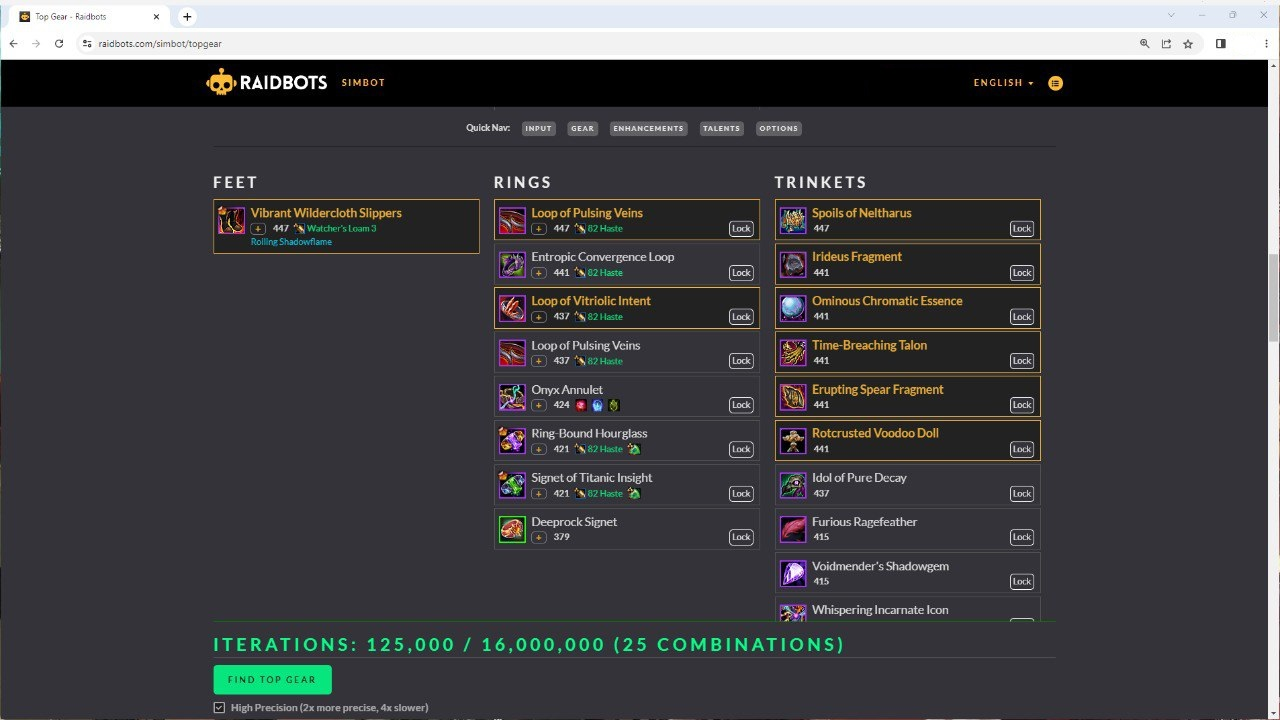
\includegraphics[width=\linewidth]{RQ1/Img/Raidbots.jpg}
    \caption{Website showing the number of all possible combinations of the gear selected by the user \cite{raider-iO-website}.}
    \label{fig:raidbots}
\end{figure}


\textbf{Discussion:} In HCI (Human Computer Interaction), Shneiderman has proposed eight golden rules \cite{shneidermans-eight-golden-rules}. 'Offer Informative Feedback' proposes offering users feedback during or immediately after an action. Such informative feedback could easily be extended with remarks about power consumption. Since power-intensive operations usually happen on the server, this does not influence the power consumption of the clients' devices. The impact of this pattern on user experience remains to be researched.


% --------------------------------------------------------------------
\subsection{Enough Resolution} \label{sec:patterns-EnoughResolution}
\textbf{Original:} ``Collect or provide high accuracy data only when strictly necessary~\cite{cruz2019catalog}."

\paragraph{Adaptation to Web}\mbox{}

\textbf{Context:} Web pages routinely collect data from web servers and provide and display this data to the user. Therefore, it is possible for web applications to collect and provide high-accuracy data only when necessary.

\textbf{Solution:} Study the importance of the collected and provided data to the user experience. Find the optimal balance between quality and size. 

\textbf{Example:} Consider a game web application. High resolution and high frame rates are necessary during game play, but when the user is in the menu, using lower frame rates is possible without reducing the overall user experience.

\textbf{Discussion:} Collection and manipulation of high-resolution data requires more resources (\eg memory, processing, capacity, etc.) than when using low resolution~\cite{cruz2019catalog}. Thus, the energy consumption is higher when processing high-resolution data.
Greenspector, a measurement and analysis solution to reduce the environmental impact of mobile and web applications, has performed a study investigating the energy impact of different image formats and resolutions on websites \cite{energy-consumption-image-format}. They found that energy consumption can be reduced by a factor of 2 for image qualities that remain high after compression and by a factor of 6 for compression to low-quality images. Chiasserini \etal~\cite{Chiasserini2002} conducted a study comparing the overall energy consumption of transmitting compressed versus non-compressed videos and still images. They show that, for example, compression of JPEG images with integer DCT kernel reduces energy costs compared to non-compressed images.

Another idea of applying this pattern to web applications could be to store, for example, several versions of the same image in different resolutions in the backend. Then the frontend can request the appropriate level of resolution depending on the use case and need not request a high-resolution image every time.


% --------------------------------------------------------------------
\subsection{Kill Abnormal Tasks} \label{sec:patterns-KillAbnormalTasks}
\textbf{Original:} ``Provide means of interrupting energy greedy operations (\eg using timeouts, or users input)~\cite{cruz2019catalog}."

\paragraph{Adaptation to Web}\mbox{}

\textbf{Context:} Timeouts are used frequently in web applications. They can be used in many different contexts. For example, session timeouts are used to handle the situation when a user does not perform any action on a website during a set interval (determined by the web server). Additionally, it is possible to offer manual means of interruption. As stated in the context of \ref{sec:patterns-InformUsers}, one of Shneidermans' eight golden rules proposes to give users informative feedback immediately after an action has been performed. It is possible to inform users of power-intensive operations and, in the same dialog, offer means of manually interrupting those operations.

\textbf{Solution:} Provide means of interrupting energy greedy operations.

\textbf{Example:} Implementation of a timeout can be seen in Listing \ref{killabnormaltaskscode}. Here, a timeout has been set to manage the calculation of different values needed to create a bill. If something goes wrong during the calculations, the timeout ensures that the abnormal behavior gets interrupted and that the resource (in this case, a worker) will be freed up again.

\begin{minipage}
    \begin{lstlisting}[caption={Example of a timeout.},label={killabnormaltaskscode}]
    some_job = django_rq.enqueue(_setup, jobs, 
            job_timeout=7200, result_ttl=1800)
    \end{lstlisting}
\end{minipage}


\textbf{Discussion:} The main concern for this pattern in mobile phones is the battery level of the device~\cite{cruz2019catalog}. In web applications, energy-intensive operations typically happen in the backend. This does not impact the energy consumption of the system through which the end user is accessing the web page. 
However, timeouts are already being used in web applications. One frequent use case is associated with a WebDriver session. Here, various timeouts control behaviors for script injection, document navigation, and element retrieval \cite{dev-mozilla-timeouts}.  Additionally, it is conceivable for developers to inform users about computation-heavy operations (see Discussion in \ref{sec:patterns-InformUsers}). In HCI, ten usability heuristics by Nielsen exist \cite{nielsen-ten-usability-heuristics}. One of which addresses user control and freedom. This heuristic states that it should always be possible for users to exit the current interaction with, for example, a cancel button. By following this suggestion, developers can ensure that any kind of interaction or task can be interrupted. Therefore, providing a means of interrupting especially energy-greedy operations would follow the usability heuristics by Nielsen.


% --------------------------------------------------------------------
\subsection{No Screen Interaction} \label{sec:patterns-NoScreenInteraction}
\textbf{Original:} ``Whenever possible allow interaction without using the display~\cite{cruz2019catalog}."

\paragraph{Adaptation to Web}\mbox{}

\textbf{Context:} Most websites require the continuous usage of the screen. There exist a few use cases where interactions can happen without using the screen (\eg allowing keyboard input to pause/start videos or to adjust volume). However, shutting down the screen while actively using a website seems only applicable to a limited number of use cases.

\textbf{Solution:} Allow users to interact with the web application using alternative interfaces (\eg keyboard input, audio).

\textbf{Example:} A website that provides an audio player could allow the screen to turn off while playing music. As an alternative interface, buttons on earphones or keyboard inputs could be used to stop/start or skip songs.

\textbf{Discussion:} One way to interact with web pages without using the screen is using a screen reader. A screen reader is part of the assistive technology (AT) that renders text and image content as speech or braille output. Users can use shortcuts on the keyboard to interact with the web pages. Popular screen readers include VoiceOver by Apple \cite{VoiceOver-Apple} and JAWS \cite{JAWS}. Such screen reader technologies have been developed for users who have visual impairments. Further research is necessary to understand the energy consumption of such assistive technology.


%---------------------------------------------------------------------

\subsection{Avoid Extraneous Graphics and Animations} \label{sec:patterns-AvoidExtraneousGraphicsAndAnimations}
\textbf{Original:} ``Graphics and animations are important for improving the user experience. However, they can also be battery intensive - use them with moderation~\cite{cruz2019catalog}."

\paragraph{Adaptation to Web}\mbox{}

\textbf{Context:} Graphics and animations can be used anywhere on a GI. Since websites provide interactive GIs, this pattern can also be applied in web applications.

\textbf{Solution:} Observe the importance of graphics and animations on the user experience. Avoid using graphics animations or high-quality graphics. If necessary, resort to low frame rates and/or low resolution.

\textbf{Example:} The company has an example of a website, that uses simple, non-animated graphics to improve the user experience.

 
\begin{comment}
\begin{figure}
     \centering
     \includegraphics[width=\linewidth]{RQ1/Img/portal_energieflüsse.png}
     \caption{Screenshot of the SEL customer portal dashboard, where simple, non-animated graphics are used to improve the user experience.}
     \label{fig:portal_energieflüsse}
 \end{figure}
\end{comment}

\textbf{Discussion:} Using graphics and animations only when they improve the user experience seems reasonable. For further explanations, also see Discussion in \ref{sec:patterns-EnoughResolution} Enough Resolution.


% --------------------------------------------------------------------
\subsection{Manual Sync, On Demand} \label{sec:patterns-ManualSyncOnDemand}
\textbf{Original:} ``Perform tasks exclusively when requested by the user~\cite{cruz2019catalog}."

\paragraph{Adaptation to Web}\mbox{}

\textbf{Context:} Some tasks, which are not strictly necessary for some application use cases, can be energy intensive.

\textbf{Solution:} Provide a mechanism that allows users to trigger energy-intensive tasks manually. For example, a button in the UI.

\textbf{Example:} The company perform actual calculations for a bill only when the user has requested it by clicking a button. They do not do operation-intensive pre-calculations on loading in case no bill was requested.

\begin{minipage}{0.95\linewidth}
  \begin{lstlisting}[caption={Implementation of a button which starts the billing process only when pressed.},label={manualsynchondemandcode}]
<template #button-bar>
<el-button
  type="primary"
  size="large"
  :loading="isBillingProcessRunning"
  @click="StartBillingCalculations"
>
  {{ $t('page.component.button.startBillingCalculations') }}
</el-button>
</template>
\end{lstlisting}
\end{minipage}

\textbf{Discussion:} Energy-intensive tasks (in the backend) do not influence the battery of the device that is visiting the website. One of the most frequently performed operations in the frontend is fetching data \ie sending requests. These requests can indeed trigger energy-intensive tasks in the backend. Shneidermans eight golden rules of interface design state, that an application should support the (users) internal locus of control \cite{shneidermans-eight-golden-rules}. This means that users need to have control and freedom so that they can feel that they are in control of the system themselves.



\section{\texorpdfstring{$RQ_2$}: Industry Insights on \EPS} 
We applied thematic analysis to developer excerpts to identify the rationale behind their concerns for \eps as shown in \autoref{fig:rq2-results-eng-patterns-motivation} and \autoref{tab:eng-patterns-motivation}.

\begin{figure}[ht]
    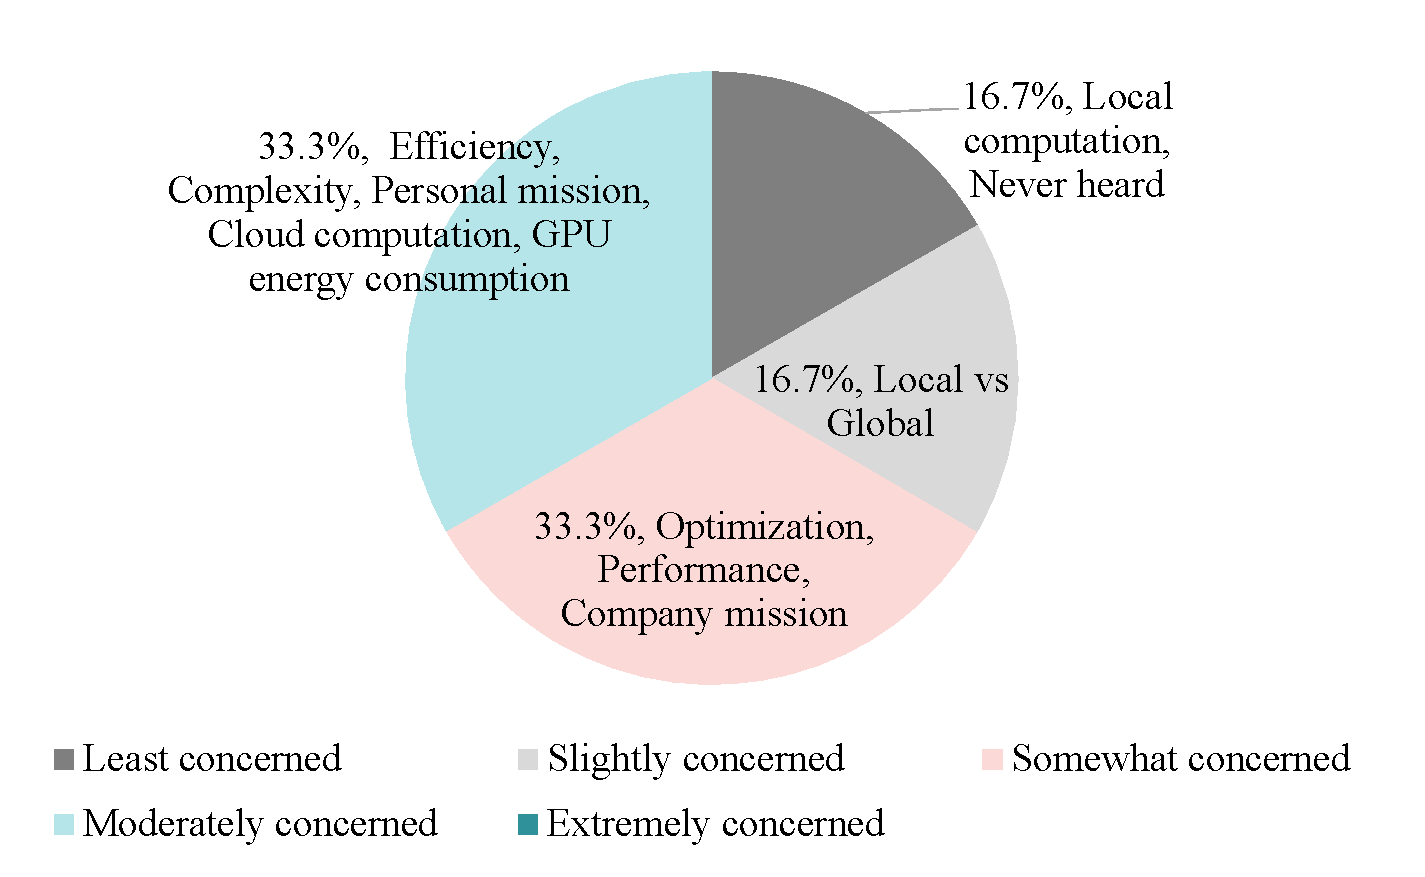
\includegraphics[width=\linewidth]{RQ2/Img/rq2-results-eng-patterns-motivation.pdf}
	\caption{Developer concerns \& motivations for patterns}
	\label{fig:rq2-results-eng-patterns-motivation}	
\end{figure}


\begin{table*}[tbh]
	\begin{center}
		\caption{ Excerpts from Developers on their motivation for \eps and corresponding codes for the motivations}
		\label{tab:eng-patterns-motivation}
		\begin{tabular}{p{0.17\textwidth}p{0.5\textwidth}p{0.29\textwidth}}
  \toprule
  			\textbf{Developers} & \textbf{Excerpts} & \textbf{Codes} \\\midrule
     P1 (moderately concerned) & \emph{\EAPS correlates with efficiency and computational complexity.} & Efficiency, Complexity
\\
P5 (somewhat concerned)                           & \emph{It depends if its locally run, or on the cloud. If local, I don't really care. If GPUs are involved or the cloud, I am more concerned because I read about energy consumption of large data centers, and I know that GPUs consume a lot of power.}   &  Local computation, Cloud computation, GPU energy consumption \\
P6 (somewhat concerned) &
\emph{Application optimization and performance are still more important than energy optimization.}
& Optimization, Performance \\

 \hline
\end{tabular}
\end{center}
\end{table*}


\section{\texorpdfstring{$RQ_3$}: Impact of \EPS} 

% \begin{figure}[ht]
	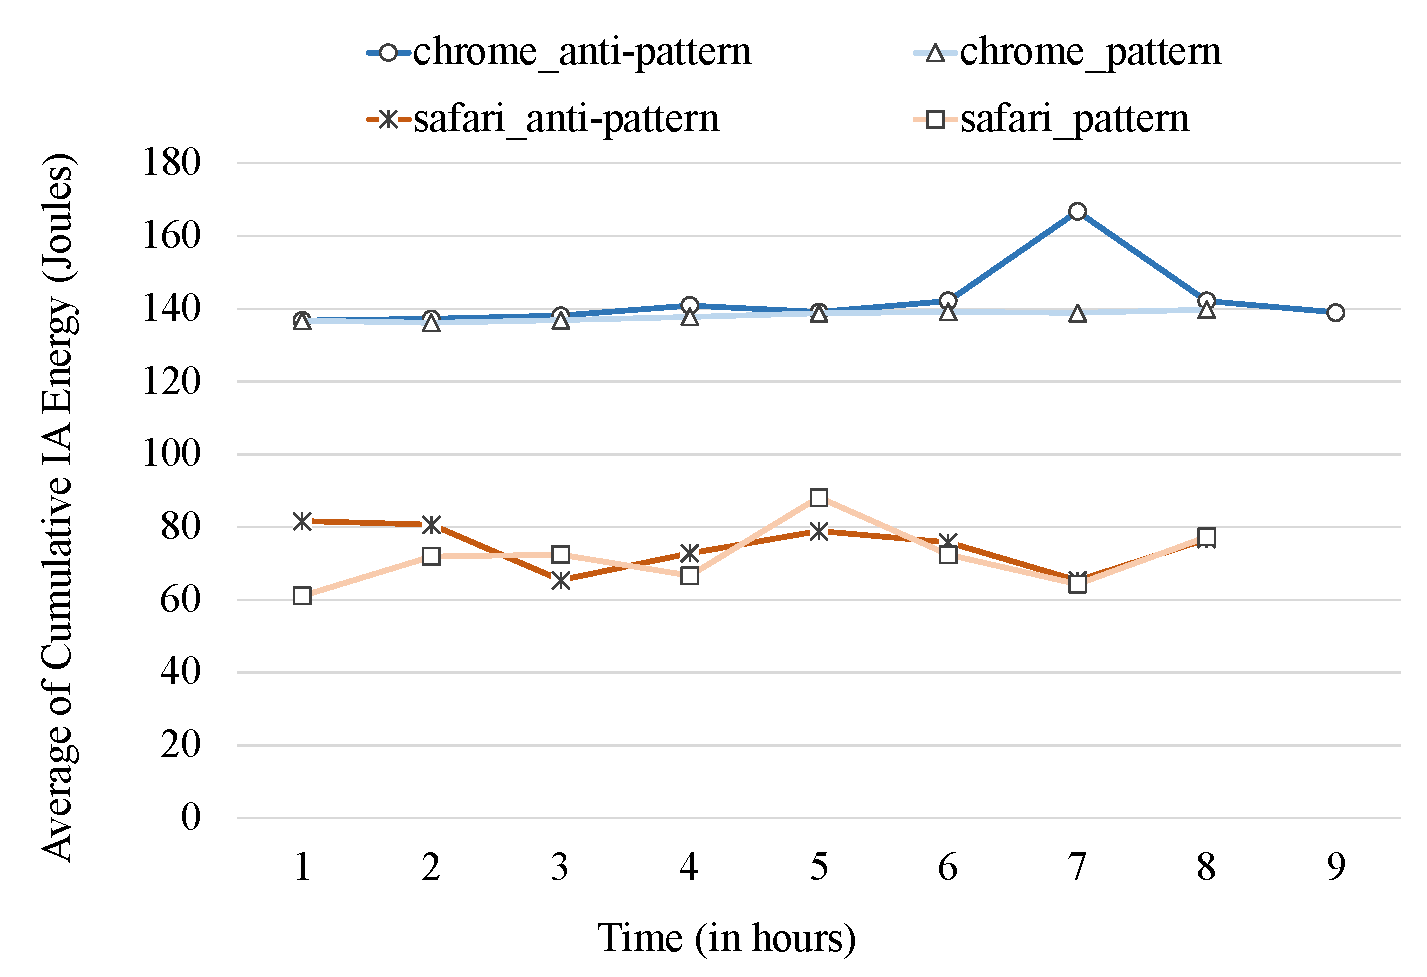
\includegraphics[width=\linewidth]{RQ3/Img/rq3-DRR-cumulative-IA-eng.pdf}
	\caption{Cumulative IA Energy for \drr}
	\label{fig:rq3-DRR-cumulative-IA-eng}	
\end{figure}
%\begin{figure}[ht]
	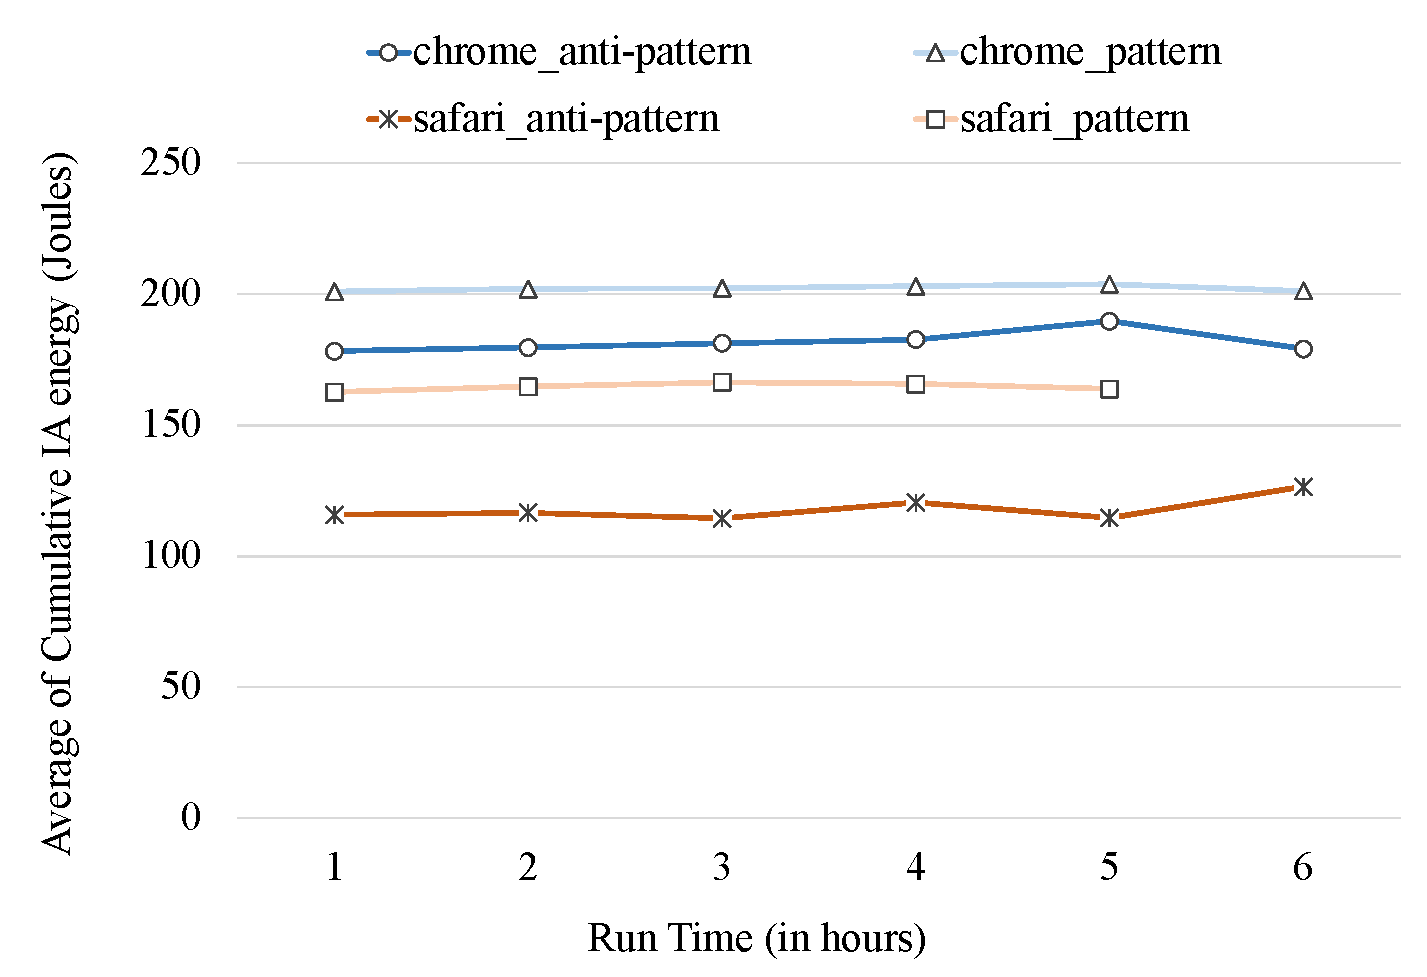
\includegraphics[width=\linewidth]{RQ3/Img/rq3-lazyload-cumulative-IA-eng.pdf}
	\caption{Cumulative IA Energy for \oown}
	\label{fig:rq3-lazyload-cumulative-IA-eng}	
\end{figure}

% \begin{figure}[ht]
 	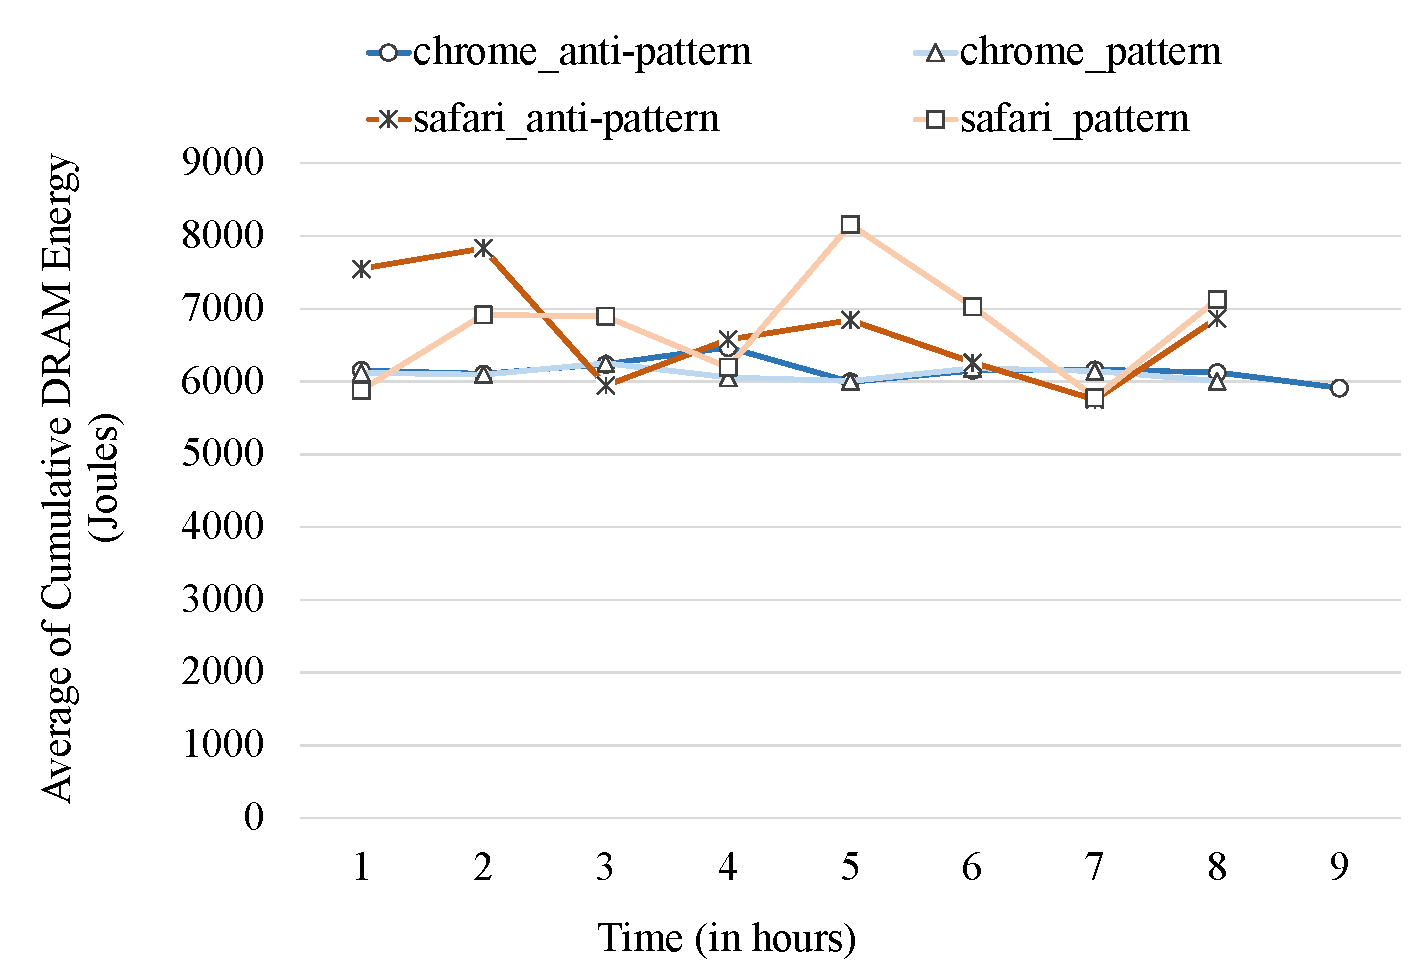
\includegraphics[width=\linewidth]{RQ3/Img/rq3-DRR-cumulative-DRAM-eng.pdf}
	\caption{DRAM energy for \drr}
	\label{fig:rq3-drr-package-eng}	
\end{figure}
% \begin{figure}[ht]
 	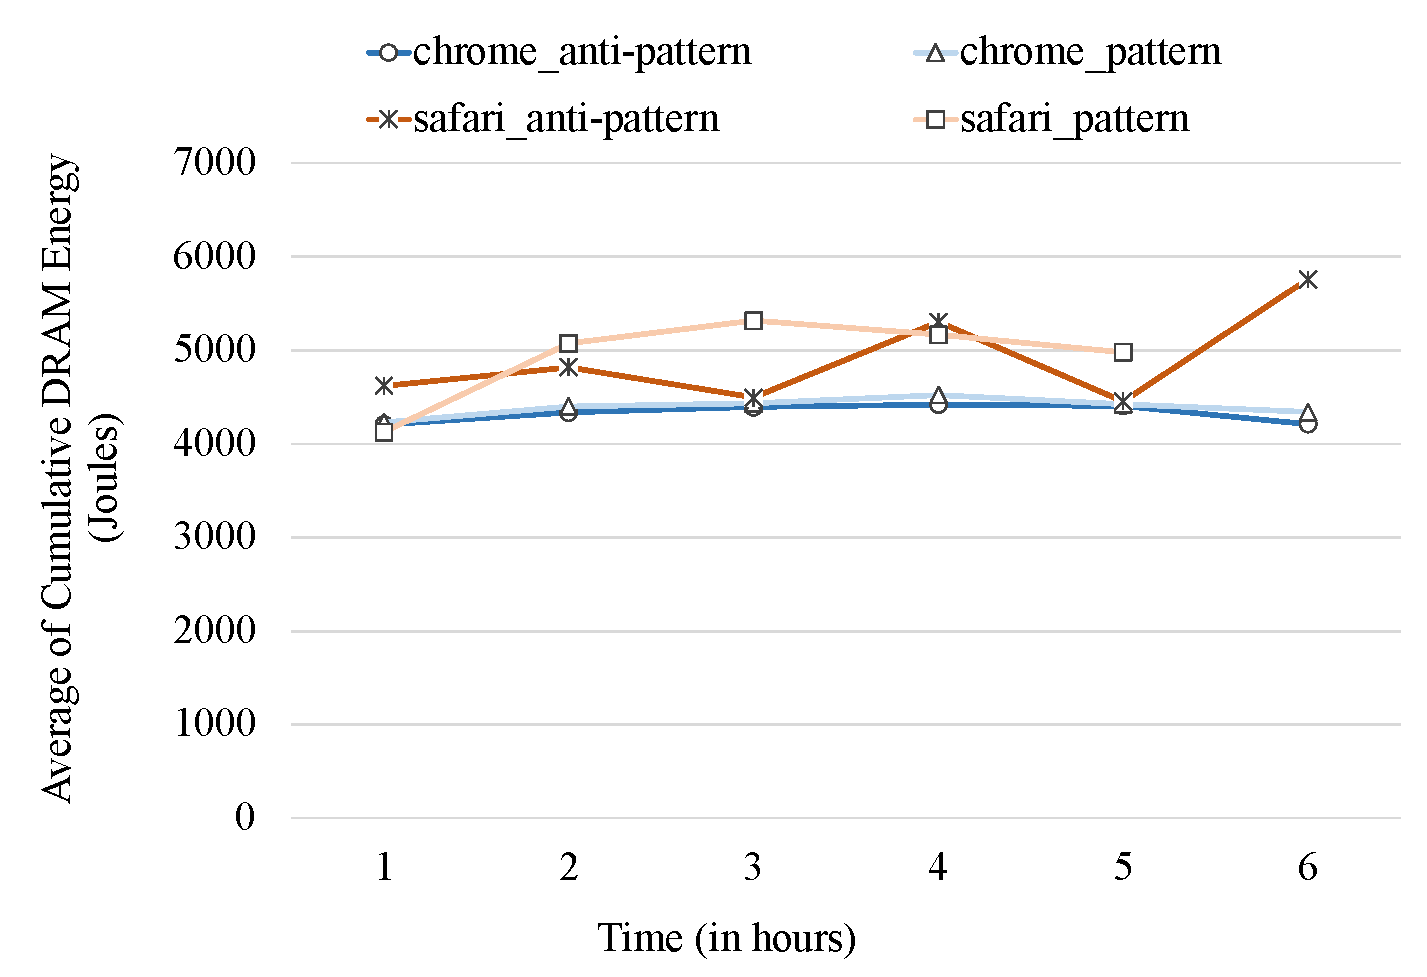
\includegraphics[width=\linewidth]{RQ3/Img/rq3-lazyload-cumulative-DRAM-eng-joul.pdf}
	\caption{DRAM energy for \oown}
	\label{fig:rq3-lazyload-package-DRAM-eng}	
\end{figure}


\bibliographystyle{ACM-Reference-Format}
\bibliography{references}
\end{document}


